\section{Methodology}
\label{sec:methodology}
% TikZ libraries for drawing shapes, arrows, and positioning
\usetikzlibrary{
    arrows.meta,
    backgrounds,
    calc,
    matrix,
    positioning,
    shapes.geometric
}

% Define colors used in the SVG diagram
\definecolor{bggray}{HTML}{f8f9fa}
\definecolor{darkblue}{HTML}{2c3e50}
\definecolor{lightbluefill}{HTML}{e3f2fd}
\definecolor{blueborder}{HTML}{1976d2}
\definecolor{lightgreenfill}{HTML}{e8f5e8}
\definecolor{greenborder}{HTML}{388e3c}
\definecolor{lightorangefill}{HTML}{fff3e0}
\definecolor{orangeborder}{HTML}{f57c00}
\definecolor{lightpurplefill}{HTML}{f3e5f5}
\definecolor{purpleborder}{HTML}{7b1fa2}
\definecolor{featureorangeborder}{HTML}{ff8f00}
\definecolor{featureorangefill}{HTML}{fff8e1}
\definecolor{redborder}{HTML}{d32f2f}
\definecolor{lightredfill}{HTML}{ffebee}
\definecolor{deeppurpleborder}{HTML}{4527a0}
\definecolor{dfrbluefill}{HTML}{e1f5fe}
\definecolor{dfrblueborder}{HTML}{0277bd}
\definecolor{backproppink}{HTML}{e91e63}
\definecolor{legendgray}{HTML}{cccccc}
\definecolor{keygray}{HTML}{666666}
\definecolor{lightgrey}{HTML}{D3D3D3}
\definecolor{lightergrey}{HTML}{F5F5F5}

\begin{figure*}[ht]
    \centering
\resizebox{0.9\linewidth}{!}{

\begin{tikzpicture}[
    font=\sffamily,
    thick,
    node distance=20mm and 25mm,
    arrowstyle/.style={-{Stealth[length=3mm, width=2.5mm]}, line width=1.8pt},
]

% == 1. DEFINE COLORS ==
\definecolor{extractorfill}{HTML}{EFEFEF}
\definecolor{blockborder}{HTML}{404040}
\definecolor{classcolor}{HTML}{B3D9FF}
\definecolor{aligncolor}{HTML}{E1D5E7}
\definecolor{lossborder}{HTML}{4472C4}
\definecolor{dfrborder}{HTML}{6A8EAE}
\definecolor{totalfill}{HTML}{FFFFFF}
\definecolor{arrowmain}{HTML}{FFC000}
\definecolor{arrowclass}{HTML}{0070C0}
\definecolor{arrowalign}{HTML}{9A009A}
\definecolor{backproppink}{HTML}{E91E63}
\definecolor{z_cell_blue}{HTML}{BDE1FB}
\definecolor{z_cell_yellow}{HTML}{FFE699}
\definecolor{dfr_item_blue}{HTML}{BDE1FB}
\definecolor{dfr_item_pink}{HTML}{E1D5E7}
\definecolor{dfr_item_yellow}{HTML}{FFE699}
\definecolor{dfr_item_green}{HTML}{C6F9C6}
\definecolor{dfr_item_red}{HTML}{F9C6C6}
% == 2. DEFINE NODE STYLES ==
\tikzset{
    inputbox/.style={rectangle, rounded corners=5pt, draw=blockborder, fill=extractorfill,minimum width=80, minimum height=40, align=center, font=\bfseries\Large},
    extractor/.style={trapezium, shape border rotate=270, trapezium left angle=70, trapezium right angle=70,
                      draw=blockborder, fill=extractorfill, minimum height=160, minimum width=60,
                      align=center, font=\bfseries\Large, line width=2.2pt},
    triangle_block/.style={isosceles triangle, shape border rotate=0, draw=blockborder,
                           minimum height=160, minimum width=100, align=center, font=\bfseries\Large},
    circle_block/.style={circle, draw=blockborder, fill=aligncolor,
                         minimum size=30mm, align=center, font=\bfseries\Large},
    lossbox/.style={rectangle, rounded corners=5pt, draw=lossborder, line width=1pt, dashed,
                    align=center, text=black, minimum height=70,
                    minimum width=70, 
                    fill=lightergrey},
    totalbox/.style={rectangle, rounded corners=8pt, draw=blockborder, fill=totalfill,minimum width=100, minimum height=50, align=center, line width=1.5pt},
    feature_vector/.style={matrix of nodes, nodes in empty cells,
                           row sep=1pt,
                           nodes={rectangle, minimum width=22pt, minimum height=10pt, draw=gray, line width=0.5pt}},
    dfr_cell/.style={rectangle, draw=dfrborder, minimum width=50mm, minimum height=6mm},
    dfr_cell_empty/.style={rectangle, draw=dfrborder, dashed, minimum width=50mm, minimum height=6mm},
}

% == 3. PLACE NODES (with input domains as images) ==

% --- MODIFIED DOMAIN BLOCKS ---
\node[rectangle, rounded corners=5pt, draw=red, line width=1.5pt,label={[font=\bfseries\Large]left:Domain 1}] (d1) at (0, 0) {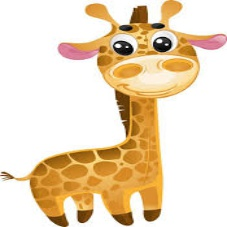
\includegraphics[width=2.5cm]{fig/giraffe_cartoon.png}};
\node[rectangle, rounded corners=5pt, draw=green, line width=1.5pt, below=5mm of d1,label={[font=\bfseries\Large]left:Domain 2}] (d2) {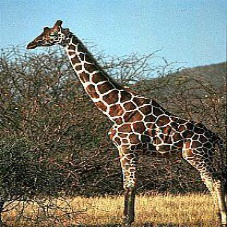
\includegraphics[width=2.5cm]{fig/giraffe_real.jpg}};
\node[font=\bfseries\Large] at ($(d2.south)!0!(d2.south)+(0,-1.5mm)$) {$\vdots$};
\node[rectangle, rounded corners=5pt, draw=blue, line width=1.5pt, below=5mm of d2,label={[font=\bfseries\Large]left:Domain N}] (d3) {
\includegraphics[width=2.5cm]{fig/giraffe_watercolor.png}};
% --- END OF MODIFICATION ---

\node[extractor, right=25mm of d2] (fe) {Feature \\ Extractor \\ ($F_\theta$)};
\matrix (z) [feature_vector, right=10mm of fe] {
    |[fill=z_cell_blue]| \\ |[fill=z_cell_yellow]| \\ |[fill=z_cell_blue]| \\
    |[fill=z_cell_blue]| \\ |[fill=z_cell_yellow]| \\ |[fill=z_cell_blue]| \\
    |[fill=z_cell_blue]| \\ |[fill=z_cell_yellow]| \\ |[fill=z_cell_blue]| \\ 
    |[fill=z_cell_blue]| \\  
};

\node[triangle_block, fill=classcolor, right=of z, yshift=3.5cm] (classifier) {Classifier \\ ($C_\psi$)};
\node[lossbox, xshift=2cm, right=of classifier] (loss_cls) {\bfseries\large $L_{\text{cls}}$};
\node[inputbox, above=5mm of loss_cls] (labels) {Labels Y};

\node[circle_block, fill=aligncolor, right=of z, yshift=-3.5cm] (l2norm) {L2 \\ Norm};
\node[lossbox, right=of l2norm, minimum width=5.5cm, minimum height=6cm] (loss_ot) {
    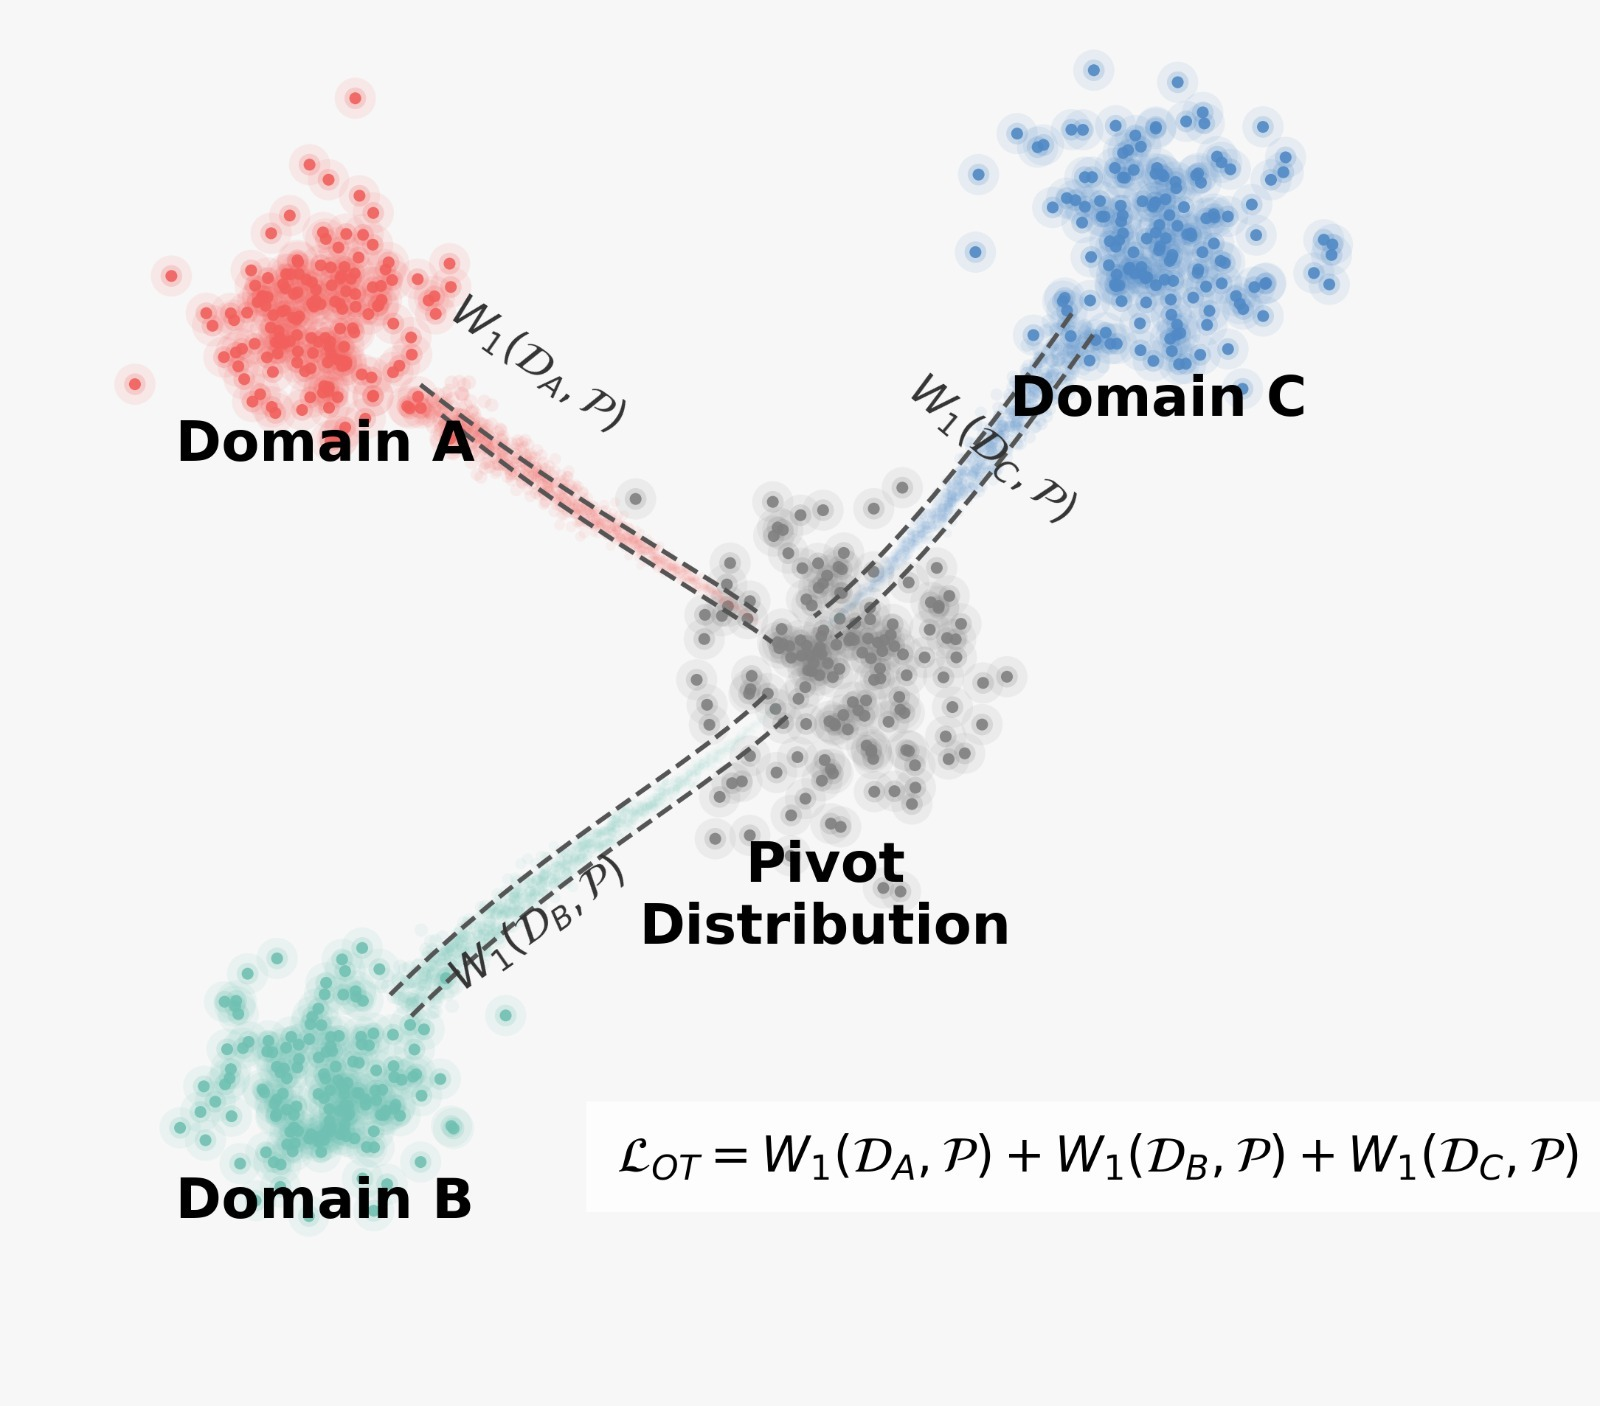
\includegraphics[width=11cm]{fig/ot_loss_plot.png} \\
    \vspace{2mm}
    \bfseries\large $L_{\text{OT}}$
};

\matrix (dfr_matrix) [matrix of nodes, below=of loss_ot, row sep=1.5pt] {
    |[dfr_cell, fill=dfr_item_blue]| \\
    |[dfr_cell, fill=dfr_item_green]| \\
    |[dfr_cell, fill=dfr_item_red]| \\
    |[dfr_cell_empty]| \\
    |[dfr_cell_empty]| \\
};
\node[fit=(dfr_matrix), draw=dfrborder, line width=1.2pt, rounded corners=3pt, inner sep=3pt] (dfr) {};
\node[below=2pt of dfr, align=center] {
      \bfseries\Large Dynamic Feature Reservoir (DFR) \\ \Large $Q \in \mathbb{R}^{K \times d}$
};

\node[totalbox, right=of loss_ot, xshift=2cm, yshift=1.5cm] (loss_total) {
    \bfseries\large $L_{\text{Total}}$ \\ \mdseries\Large $= L_{\text{cls}} + \lambda L_{\text{OT}}$
};

% == 4. DRAW ARROWS AND CONNECTIONS ==

\draw[arrowstyle, draw=black!70] (d1.east) -- (fe.west);
\draw[arrowstyle, draw=black!70] (d2.east) -- (fe.west);
\draw[arrowstyle, draw=black!70] (d3.east) -- (fe.west);
\draw[arrowstyle, draw=arrowmain] (fe.east) -- (z.west) node[midway, above, font=\bfseries\color{arrowmain}] {Z};

\coordinate (z_split_point) at ($(z.east)$);

\draw[arrowstyle, draw=arrowclass] (z_split_point) to[out=45, in=180] (classifier.west);
\draw[arrowstyle, draw=arrowalign] (z_split_point) to[out=-45, in=180] (l2norm.west);

\draw[arrowstyle, draw=arrowclass] (classifier.east) -- (loss_cls.west);
\draw[arrowstyle, draw=arrowclass] (labels.south) -- (loss_cls.north);
\draw[arrowstyle, draw=arrowalign] (l2norm.east) -- (loss_ot.west);

\draw[arrowstyle, draw=dfrborder, line width=1.5pt] (dfr.north) -- (loss_ot.south) node[midway, right, font=\small]{Read};
\draw[arrowstyle, draw=arrowalign, dashed] (l2norm.south) |- (dfr.west) node[midway, above right, font=\small]{Update};

\draw[arrowstyle, draw=black!60] (loss_cls.east) to[out=0, in=140] (loss_total.west);
\draw[arrowstyle, draw=black!60] (loss_ot.east) to[out=0, in=220] (loss_total.west);

\draw[arrowstyle, draw=backproppink, dashed] (loss_total.north) to[out=90, in=0] ($(loss_total.north) + (-6cm,10cm)$) to[out=180, in=90] ($(fe.north) + (0,1cm)$) to[out=270, in=90] (fe.north);

% == 5. LEGEND ==
\begin{scope}[node distance=2mm, font=\sffamily\small, text=black,
              every node/.style={anchor=west}]
    \node[draw=black!40, fill=white, rounded corners=5pt,
          left=of dfr, xshift=-10cm, align=left] (legend_box) {
        \begin{tabular}{p{1.5cm} l}
            \tikz\draw[arrowstyle, draw=arrowclass] (0,0) -- (1,0); & Classification path \\
            \tikz\draw[arrowstyle, draw=arrowalign] (0,0) -- (1,0); & Alignment path \\
            \tikz\draw[arrowstyle, draw=arrowalign, dashed] (0,0) -- (1,0); & Update (no gradients) \\
            \tikz\draw[arrowstyle, draw=backproppink, dashed] (0,0) -- (1,0); & Backpropagation \\
            \tikz\draw[arrowstyle, draw=dfrborder] (0,0) -- (1,0); & DFR read operation \\
        \end{tabular}
    };
\end{scope}

\end{tikzpicture}
} % End of resizebox
\caption{Overview of SODA. The framework consists of a standard supervised path (\textcolor{blue}{blue}) and a stabilized OT alignment path (\textcolor{purple}{purple}). Crucially, the Dynamic Feature Reservoir (DFR) is updated via a gradient-free queue mechanism (dashed line), ensuring it acts as a stable anchor. The alignment loss $\mathcal{L}_{OT}$ minimizes the entropic OT cost between the current mini-batch features and the non-parametric distribution defined by the reservoir.}
\label{fig:soda_framework}    
\end{figure*}

This section presents the SODA (\underline{S}tabilized \underline{O}ptimal Transport Based \underline{D}omain \underline{A}lignment) framework, illustrated in Figure~\ref{fig:soda_framework}. We begin with mathematical preliminaries for Domain Generalization and Optimal Transport theory. We then formally characterize the pivot instability problem and introduce our solution: the Dynamic Feature Reservoir (DFR). Finally, we present the complete SODA algorithm and analyze its computational properties.

\subsection{Problem Formulation}
\label{ssec:problem}

The objective in Domain Generalization (DG) is to learn a model that generalizes from a set of source domains to an unseen target domain. Let $\mathcal{D}_S = \{D_1, D_2, \dots, D_N\}$ be $N$ source domains, where each domain $D_i$ is characterized by a distribution $P_i(X, Y)$ over input space $\mathcal{X} \subset \mathbb{R}^d$ and label space $\mathcal{Y} = \{1, \dots, C\}$. The domain shift assumption states that marginal distributions differ across domains ($P_i(X) \neq P_j(X)$ for $i \neq j$), while the labeling function $P(Y|X)$ remains consistent. The goal is to learn a model from $\mathcal{D}_S$ that performs well on an unseen target domain $D_t$ with distribution $P_t(X, Y)$.

We decompose the model $h: \mathcal{X} \to \mathcal{Y}$ into a feature extractor $f_\theta: \mathcal{X} \to \mathcal{Z}$ mapping inputs to a latent space $\mathcal{Z} \subset \mathbb{R}^{d'}$, and a classifier $C_\psi: \mathcal{Z} \to \mathbb{R}^C$ mapping features to class logits. The expected risk on a domain with distribution $P(X,Y)$ is:
\begin{equation}
    R(f_\theta, C_\psi) := \mathbb{E}_{(x,y) \sim P(X,Y)} [\mathcal{L}(C_\psi(f_\theta(x)), y)].
\end{equation}

Since the target distribution $P_t$ is inaccessible during training, the standard approach is Empirical Risk Minimization (ERM), which minimizes average risk across source domains:
\begin{equation}
    \mathcal{L}_{\text{ERM}}(\theta, \psi) = \frac{1}{N} \sum_{i=1}^{N} \mathbb{E}_{(x,y) \sim P_i(X,Y)} [\mathcal{L}_{\text{CE}}(C_\psi(f_\theta(x)), y)],
    \label{eq:erm}
\end{equation}
where $\mathcal{L}_{\text{CE}}$ denotes Cross-Entropy loss. However, ERM may overfit to domain-specific correlations. Domain alignment methods address this by adding a regularization term $\mathcal{L}_{\text{align}}$ that penalizes discrepancies between feature distributions $P_i(Z)$ where $Z = f_\theta(X)$.

An ideal alignment objective would minimize pairwise discrepancies between all source feature distributions:
\begin{equation}
    \mathcal{L}_{\text{align-ideal}}(\theta) = \frac{1}{N(N-1)} \sum_{i \neq j} d(P_i(Z), P_j(Z)),
\end{equation}
where $d(\cdot, \cdot)$ is a discrepancy measure. This objective requires $\binom{N}{2}$ comparisons, yielding $\mathcal{O}(N^2)$ complexity per step. A tractable alternative introduces a pivot distribution $P_{\text{pivot}}$:
\begin{equation}
    \mathcal{L}_{\text{align}}(\theta) = \frac{1}{N} \sum_{i=1}^{N} d(P_i(Z), P_{\text{pivot}}),
\end{equation}
reducing complexity to $\mathcal{O}(N)$. The total training objective becomes:
\begin{equation}
    \label{eq:dg_objective}
    \mathcal{L}_{\text{Total}}(\theta, \psi) = \mathcal{L}_{\text{ERM}}(\theta, \psi) + \lambda \mathcal{L}_{\text{align}}(\theta),
\end{equation}
where $\lambda$ balances classification and alignment. The effectiveness of this strategy depends critically on (1) the discrepancy measure $d(\cdot, \cdot)$, and (2) the statistical properties of $P_{\text{pivot}}$.

\subsection{Optimal Transport Theory}
\label{ssec:ot_foundations}

\begin{figure}[t]
    \centering
    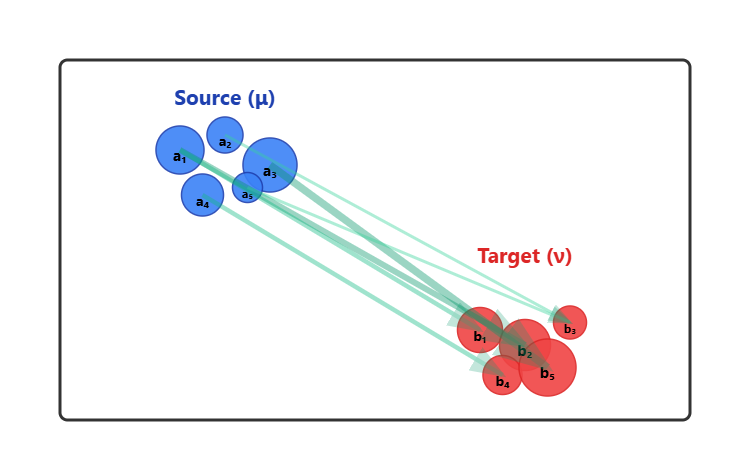
\includegraphics[width=0.8\textwidth]{fig/OT_Illustration.png}
    \caption{Optimal Transport illustration. (a) Two discrete probability measures: source $\mu$ and target $\nu$, where point size indicates mass. (b) The optimal transport plan $T^*$ describes mass flow from source to target, minimizing total transportation cost. Line thickness indicates transported mass.}
    \label{fig:ot_concept}
\end{figure}

We adopt Optimal Transport (OT) as our discrepancy measure for its geometric properties. OT finds the most efficient coupling that transforms a source measure $\mu$ into a target measure $\nu$ while minimizing transportation cost (Figure~\ref{fig:ot_concept}). Rooted in the work of Monge and Kantorovich~\citep{villani2009optimal}, OT computes the minimal effort to transform one distribution into another, which is particularly suited for comparing feature manifolds with non-overlapping supports where divergence-based measures may fail.

\subsubsection{Discrete Optimal Transport}
\begin{sloppypar} 
For discrete distributions $\mu$ and $\nu$ supported on feature vectors $\{z_1, \dots, z_m\} \subset \mathcal{Z}$ and $\{z'_1, \dots, z'_n\} \subset \mathcal{Z}$ with probability vectors $\mathbf{a} \in \Delta_m$ and $\mathbf{b} \in \Delta_n$, where the probability simplex is defined as:
\begin{equation}
    \Delta_k := \left\{ \mathbf{p} \in \mathbb{R}^k_+ \ \Big| \ \sum_{i=1}^{k} p_i = 1 \right\},
\end{equation}
we define the ground cost matrix $\mathbf{M} \in \mathbb{R}^{m \times n}$ with entries:
\begin{equation}
    \label{eq:cost}
    M_{ij} = c(z_i, z'_j) = \|z_i - z'_j\|_2^2,
\end{equation}
where we use squared Euclidean distance as the cost function.
\end{sloppypar} 
A transport plan $\mathbf{T} \in \mathbb{R}^{m \times n}_+$ specifies the mass $T_{ij}$ transported from source point $z_i$ to target point $z'_j$. Valid transport plans must satisfy marginal constraints, forming the transport polytope:
\begin{equation}
    \Pi(\mathbf{a}, \mathbf{b}) := \left\{ \mathbf{T} \in \mathbb{R}^{m \times n}_+ \ \Big| \ \mathbf{T}\mathbf{1}_n = \mathbf{a}, \ \mathbf{T}^\top\mathbf{1}_m = \mathbf{b} \right\},
\end{equation}
where $\mathbf{1}_k$ denotes the $k$-dimensional vector of ones. The constraint $\mathbf{T}\mathbf{1}_n = \mathbf{a}$ ensures mass conservation at each source point, while $\mathbf{T}^\top\mathbf{1}_m = \mathbf{b}$ ensures each target point receives its prescribed mass.

The Kantorovich formulation seeks the optimal plan minimizing total transportation cost:
\begin{equation}
    \mathcal{L}_{\mathbf{M}}(\mu, \nu) = \min_{\mathbf{T} \in \Pi(\mathbf{a}, \mathbf{b})} \langle \mathbf{T}, \mathbf{M} \rangle_F = \min_{\mathbf{T} \in \Pi(\mathbf{a}, \mathbf{b})} \sum_{i,j} T_{ij} M_{ij},
\end{equation}
where $\langle \cdot, \cdot \rangle_F$ denotes the Frobenius inner product. This linear program has complexity $\mathcal{O}(n^3 \log n)$ via network simplex algorithms, which is prohibitive for deep learning.

\subsubsection{Entropic Regularization and the Sinkhorn Algorithm}

To enable efficient computation, we adopt entropic regularization~\citep{cuturi2013sinkhorn}, which introduces a strictly convex penalty:
\begin{equation}
    \label{eq:entropic_ot}
    \mathcal{L}^\epsilon_{\mathbf{M}}(\mu, \nu) = \min_{\mathbf{T} \in \Pi(\mathbf{a}, \mathbf{b})} \langle \mathbf{T}, \mathbf{M} \rangle_F - \epsilon H(\mathbf{T}),
\end{equation}
where $\epsilon > 0$ is the regularization strength and $H(\mathbf{T})$ is the entropy of the transport plan:
\begin{equation}
    H(\mathbf{T}) = -\sum_{i,j} T_{ij}(\log T_{ij} - 1).
\end{equation}

To derive the solution, we form the Lagrangian with dual variables $\boldsymbol{\alpha} \in \mathbb{R}^m$ and $\boldsymbol{\beta} \in \mathbb{R}^n$ for the marginal constraints:
\begin{equation}
    \mathcal{L}(\mathbf{T}, \boldsymbol{\alpha}, \boldsymbol{\beta}) = \langle \mathbf{T}, \mathbf{M} \rangle_F - \epsilon H(\mathbf{T}) - \langle \boldsymbol{\alpha}, \mathbf{T}\mathbf{1}_n - \mathbf{a} \rangle - \langle \boldsymbol{\beta}, \mathbf{T}^\top\mathbf{1}_m - \mathbf{b} \rangle.
\end{equation}

Setting $\frac{\partial \mathcal{L}}{\partial T_{ij}} = 0$ yields the first-order optimality condition:
\begin{equation}
    M_{ij} + \epsilon \log T^*_{ij} - \alpha_i - \beta_j = 0,
\end{equation}
which gives the optimal transport plan in closed form:
\begin{equation}
    \label{eq:optimal_plan_form}
    T^*_{ij} = \exp\left(\frac{\alpha_i + \beta_j - M_{ij}}{\epsilon}\right) = \exp\left(\frac{\alpha_i}{\epsilon}\right) \exp\left(\frac{-M_{ij}}{\epsilon}\right) \exp\left(\frac{\beta_j}{\epsilon}\right).
\end{equation}

Defining scaling vectors $\mathbf{u} = e^{\boldsymbol{\alpha}/\epsilon} \in \mathbb{R}^m_+$ and $\mathbf{v} = e^{\boldsymbol{\beta}/\epsilon} \in \mathbb{R}^n_+$, and the Gibbs kernel $\mathbf{K} = e^{-\mathbf{M}/\epsilon}$ with entries $K_{ij} = e^{-M_{ij}/\epsilon}$, we obtain the matrix factorization:
\begin{equation}
    \mathbf{T}^*_\epsilon = \text{diag}(\mathbf{u}) \, \mathbf{K} \, \text{diag}(\mathbf{v}).
\end{equation}

The scaling vectors are determined by the marginal constraints. Substituting into $\mathbf{T}\mathbf{1}_n = \mathbf{a}$ and $\mathbf{T}^\top\mathbf{1}_m = \mathbf{b}$ yields the Sinkhorn-Knopp fixed-point equations:
\begin{equation}
    \mathbf{u} = \frac{\mathbf{a}}{\mathbf{K}\mathbf{v}}, \quad \mathbf{v} = \frac{\mathbf{b}}{\mathbf{K}^\top\mathbf{u}},
\end{equation}
where division is element-wise. Starting from $\mathbf{v}^{(0)} = \mathbf{1}_n$, the algorithm iterates:
\begin{equation}
    \mathbf{u}^{(l+1)} = \frac{\mathbf{a}}{\mathbf{K}\mathbf{v}^{(l)}}, \quad \mathbf{v}^{(l+1)} = \frac{\mathbf{b}}{\mathbf{K}^\top\mathbf{u}^{(l+1)}}.
\end{equation}

This algorithm converges linearly with rate dependent on $\epsilon$~\citep{peyre2019computational}. We denote the resulting \emph{entropic OT cost} by $W_\epsilon(\mu, \nu) := \mathcal{L}^\epsilon_{\mathbf{M}}(\mu, \nu)$; it is differentiable with respect to input feature locations, enabling end-to-end training. $W_\epsilon$ differs from the (debiased) Sinkhorn divergence $S_\epsilon(\mu,\nu)=W_\epsilon(\mu,\nu)-\tfrac12W_\epsilon(\mu,\mu)-\tfrac12W_\epsilon(\nu,\nu)$~\citep{feydy2019interpolating}, which removes the entropic bias so that $S_\epsilon(\mu,\mu)=0$. SODA minimizes $W_\epsilon$: our implementation uses GeomLoss~\citep{feydy2019interpolating} with \texttt{debias=False}, ground cost $\tfrac12\|x-y\|^2$ and $\epsilon=\texttt{blur}^2$, which yields the same transport plans as Eq.~(\ref{eq:entropic_ot}) with $\epsilon=2\,\texttt{blur}^2$ and half its value. Replacing $W_\epsilon$ by $S_\epsilon$ does not change accuracy in our experiments (70.8\% with either loss on OfficeHome over three seeds).

\subsubsection{Gradient Flow and Feature Learning}

A key property for our application is how $W_\epsilon$ induces gradients on feature representations. The transport polytope $\Pi(\mathbf a,\mathbf b)$ does not depend on the support points and the entropic problem has a unique solution $\mathbf T^*_\epsilon$, so by the envelope theorem the gradient with respect to a source feature $z_i$, for the squared Euclidean cost of Eq.~(\ref{eq:cost}), is~\citep{peyre2019computational}:
\begin{equation}
    \label{eq:wasserstein_gradient}
    \nabla_{z_i} W_\epsilon(\mu, \nu) = 2 \sum_{j=1}^{n} T^*_{ij} (z_i - z'_j) = 2a_i\big(z_i-\hat z_i\big),\qquad \hat z_i:=\frac{1}{a_i}\sum_{j=1}^n T^*_{ij}z'_j .
\end{equation}

This gradient pulls $z_i$ toward $\hat z_i$, a weighted average of the target points matched to it, with weights given by the transport plan. Minimizing $W_\epsilon$ thus moves source features toward their optimal correspondences in the target distribution. There is no explicit $1/\epsilon$ factor: $\epsilon$ acts only through $\mathbf T^*_\epsilon$. Smaller $\epsilon$ concentrates each row of the plan on a few nearby target points, so the gradient depends on individual target samples; larger $\epsilon$ spreads it over many, and as $\epsilon\to\infty$ the plan tends to $\mathbf a\mathbf b^\top$ and the gradient only matches means. For unit-norm features the gradient norm is at most $4a_i$ for every $\epsilon$.

\subsubsection{Effect of Entropic Regularization on Transport Plans}

The parameter $\epsilon$ fundamentally affects the structure of $\mathbf{T}^*_\epsilon$:

\begin{proposition}[Transport Plan Entropy]
\label{prop:entropy}
As $\epsilon \to 0$, the optimal plan $\mathbf{T}^*_\epsilon$ converges to the sparse solution of the unregularized problem, approaching a permutation matrix for equal-mass distributions. As $\epsilon \to \infty$, $\mathbf{T}^*_\epsilon \to \mathbf{a}\mathbf{b}^\top$, the maximum-entropy independent coupling.
\end{proposition}

This has important implications for domain alignment:
\begin{itemize}
    \item \textbf{Low $\epsilon$}: Sparse plans create hard assignments between source and target features. Gradients are dominated by nearest-neighbor correspondences, making optimization sensitive to outliers and local density variations.
    \item \textbf{High $\epsilon$}: Dense plans distribute mass broadly, creating soft many-to-many alignments. Each source feature receives gradient contributions from multiple target features, providing implicit regularization against overfitting to specific target samples.
\end{itemize}

The reservoir contains features encoded by earlier parameters; Section~\ref{ssec:dfr} bounds the resulting bias (Proposition~\ref{prop:staleness}) and Section~\ref{sec:stability_analysis} measures it during training.

\subsection{The Pivot Instability Problem}
\label{ssec:pivot_instability}

Applying OT to multi-source DG requires a pivot distribution $P_{\text{pivot}}$ for alignment. Conventional approaches construct this pivot from the current minibatch, either using a randomly selected source domain's features or pooling all minibatch features: $P_{\text{pivot}} = \text{Uniform}(\{z_k\}_{k=1}^{B})$. Both strategies suffer from \textit{pivot instability}: the target distribution fluctuates substantially across iterations due to stochastic sampling.

\subsubsection{Formal Definition of Stability}

We formally characterize pivot stability in terms of the divergence between consecutive pivot distributions:

\begin{definition}[Pivot Stability]
\label{def:stability}
Let $P_{\text{pivot}}^{(t)}$ denote the pivot distribution at training iteration $t$. The \textit{pivot instability} $\mathcal{S}$ is the expected Wasserstein distance between consecutive pivots:
\begin{equation}
    \mathcal{S} := \mathbb{E}_t\left[W_2\left(P_{\text{pivot}}^{(t)}, P_{\text{pivot}}^{(t+1)}\right)\right].
\end{equation}
A pivot mechanism with lower $\mathcal{S}$ provides more consistent optimization targets.
\end{definition}

For batch-derived pivots reconstructed entirely each iteration, $\mathcal{S}$ equals the expected Wasserstein distance between independent samples from the feature distribution—which can be substantial in high-dimensional spaces.

\subsubsection{Impact on Gradient Variance}

Pivot instability directly affects the variance of the alignment gradient. Let $\mathbf{g}^{(t)} = \nabla_\theta \mathcal{L}_{\text{align}}^{(t)}$ denote the alignment gradient at iteration $t$. We can decompose:
\begin{equation}
    \text{Var}[\mathbf{g}^{(t)}] = \underbrace{\text{Var}[\mathbf{g}^{(t)} | P_{\text{pivot}}]}_{\text{Source sampling variance}} + \underbrace{\mathbb{E}[\text{Var}[\mathbf{g}^{(t)} | P_{\text{source}}]]}_{\text{Pivot variance}}.
\end{equation}

The first term arises from stochastic sampling of source features and is irreducible given batch size constraints. The second term arises from pivot fluctuations and can be controlled through pivot design. High pivot variance manifests as conflicting gradient directions across iterations, hindering convergence.

\subsubsection{Statistical Impossibility in High Dimensions}

The instability problem is exacerbated by a fundamental statistical limitation. \citet{dong2025distribution} establish an impossibility result for distribution matching from small samples:

\begin{theorem}[Informal, from \citet{dong2025distribution}]
\label{thm:impossibility}
If feature dimension $d'$ exceeds batch size $B$ plus one (i.e., $d' > B + 1$), then for any minibatch $\{z_1, \dots, z_B\}$, there exist infinitely many distinct distributions that assign identical likelihood to that minibatch.
\end{theorem}

With typical configurations ($d' = 2048$ for ResNet-50, $B = 32$), batch-derived pivot distributions are statistically ambiguous. The optimization signal reflects sampling artifacts rather than true distributional structure, causing the model to align spurious correlations.

\subsection{The Dynamic Feature Reservoir}
\label{ssec:dfr}

To address pivot instability, we introduce the Dynamic Feature Reservoir (DFR), which decouples the pivot's effective sample size from the training batch size.

\subsubsection{Reservoir Definition and Update}

The DFR is a matrix $\mathbf{Q} \in \mathbb{R}^{K \times d'}$ storing $K$ L2-normalized feature vectors, where $K \gg B$. The empirical distribution over its rows defines the pivot:
\begin{equation}
    P_{\mathbf{Q}} = \frac{1}{K} \sum_{k=1}^{K} \delta_{\mathbf{q}_k},
\end{equation}
where $\delta_{\mathbf{q}_k}$ is the Dirac measure at the $k$-th row of $\mathbf{Q}$.

The reservoir is updated after each training step via first-in-first-out (FIFO) insertion. A pointer $\text{ptr} \in \{0, 1, \dots, K-1\}$ tracks the insertion position. For each feature $z$ in the current minibatch:
\begin{equation}
    \mathbf{Q}[\text{ptr}] \leftarrow \frac{z}{\|z\|_2}, \quad \text{ptr} \leftarrow (\text{ptr} + 1) \mod K.
\end{equation}

This update is gradient-free: features are detached from the computational graph before insertion, preventing degenerate solutions where the reservoir collapses to match arbitrary source features.

\subsubsection{Stability Analysis}

The DFR achieves stability through its large capacity relative to batch size. At each iteration, only the $B$ entries inserted by Algorithm~\ref{alg:sota} change, a fraction $B/K$ of the reservoir:

\begin{proposition}[DFR Stability]
\label{prop:dfr_stability}
Let $\mathbf Q^{(t)},\mathbf Q^{(t+1)}\in(\mathbb S^{d'-1})^K$ be consecutive reservoirs that differ in $B\le K$ rows, and let $P_{\mathbf Q}^{(t)},P_{\mathbf Q}^{(t+1)}$ be their uniform empirical measures. Then, for every $p\ge1$,
\begin{equation}
    W_p\big(P_{\mathbf Q}^{(t)},P_{\mathbf Q}^{(t+1)}\big)\le\Big(\frac1K\sum_{k\in R_t}\big\|q^{(t)}_k-q^{(t+1)}_k\big\|^p\Big)^{1/p}\le2\Big(\frac BK\Big)^{1/p},
\end{equation}
where $R_t$ is the set of overwritten rows. In particular $\mathcal S_{\text{DFR}}\le2\sqrt{B/K}$ for the $W_2$ instability of Definition~\ref{def:stability}, and $W_1\le2B/K$; both bounds are attained. Moreover, for any source measure $\alpha$ on the unit sphere and any $\epsilon\ge0$, $\big|W_\epsilon(\alpha,P_{\mathbf Q}^{(t+1)})-W_\epsilon(\alpha,P_{\mathbf Q}^{(t)})\big|\le4B/K$.
\end{proposition}
\begin{proof}
The coupling that is the identity on the $K-B$ shared rows and pairs each overwritten row with the row that replaces it is feasible, since all atoms have mass $1/K$. Its cost is $\frac1K\sum_{k\in R_t}\|q^{(t)}_k-q^{(t+1)}_k\|^p\le\frac BK2^p$ because the unit sphere has diameter $2$, which gives both inequalities; equality holds when all overwritten rows equal $e$ and all new rows equal $-e$. For the last claim, the optimal plan for $(\alpha,P_{\mathbf Q}^{(t)})$ is feasible for $(\alpha,P_{\mathbf Q}^{(t+1)})$ with the same entropy; its cost changes only on the overwritten columns, of total mass $B/K$, by at most $4=\max\|x-y\|^2$ each. Exchanging $t$ and $t+1$ completes the proof.
\end{proof}

The Wasserstein-2 distance between consecutive reservoirs therefore scales with $\sqrt{B/K}$, while the change of the loss scales linearly with $B/K$. With $K=512$ and $B=96$ features per step (32 per source domain), $\mathcal S_{\text{DFR}}\le0.87$. A batch-derived pivot is redrawn at every step and shares no points with its predecessor, so its drift does not decrease with $K$; Section~\ref{sec:stability_analysis} measures both.

\subsubsection{Gradient Variance Reduction}

The stability improvement directly reduces gradient variance. From Equation~\ref{eq:wasserstein_gradient}, the alignment gradient depends on the transport plan $\mathbf{T}^*$, which in turn depends on the target distribution. With a stable pivot:

\begin{proposition}[Gradient Variance Bound]
\label{prop:gradient_variance}
Let $\mathbf{g}_{\text{batch}}^{(t)}$ and $\mathbf{g}_{\text{DFR}}^{(t)}$ denote alignment gradients using batch-derived and DFR pivots respectively. Under mild regularity conditions on the feature distribution:
\begin{equation}
    \text{Var}\left[\mathbf{g}_{\text{DFR}}^{(t)}\right] \leq \text{Var}\left[\mathbf{g}_{\text{batch}}^{(t)}\right] - \Omega\left(\frac{K-B}{K}\right) \cdot \sigma^2_{\text{pivot}},
\end{equation}
where $\sigma^2_{\text{pivot}}$ is the variance contribution from pivot fluctuations.
\end{proposition}

This reduced variance enables more consistent optimization, as the feature extractor receives coherent gradient signals across iterations rather than conflicting directions caused by pivot fluctuations.

\subsubsection{Sample Complexity Considerations}

The DFR also addresses the statistical impossibility of Theorem~\ref{thm:impossibility} by increasing effective sample size. \citet{genevay2019sample} establish that, for measures supported on a bounded set $\mathcal X\subset\mathbb R^d$ and a smooth Lipschitz cost, the sample complexity of the entropic OT cost (and of the Sinkhorn divergence) scales as:
\begin{equation}
    \mathbb{E}\left[|W_\epsilon(\hat{\mu}_n, \hat{\nu}_m) - W_\epsilon(\mu, \nu)|\right] = \mathcal{O}\left(\frac{e^{\kappa/\epsilon}}{\sqrt{\min(n,m)}}\Big(1+\frac{1}{\epsilon^{\lfloor d/2\rfloor}}\Big)\right),
\end{equation}
where $\hat{\mu}_n, \hat{\nu}_m$ are empirical distributions with $n$ and $m$ samples respectively and $\kappa$ depends on the diameter of $\mathcal X$ and the cost. In high dimension the constant is large, so the bound is qualitative.

For SODA, the source distribution has $B$ samples while the target (DFR) has $K$ samples. The estimation error is thus dominated by $B$ and does not improve once $K \geq B$. What the reservoir changes is the variation of the pivot, and hence of the alignment gradient, across training iterations, which we measure directly in Section~\ref{sec:stability_analysis}.

\subsubsection{Design Properties}

The DFR provides three complementary properties:

\textbf{Stability.} With $K \gg B$, the pivot evolves slowly, providing consistent optimization targets across iterations. Each entry keeps weight $1/K$ for exactly $\lceil K/B\rceil$ steps and is then removed.

\textbf{Adaptivity.} The FIFO mechanism ensures the reservoir incorporates improving features as training progresses while discarding stale representations. After $A:=\lceil K/B\rceil$ iterations, the entire reservoir has been refreshed. The bias caused by stale entries is therefore bounded by the feature drift over the last $A$ steps:

\begin{proposition}[Staleness bias]
\label{prop:staleness}
Let entry $k$ of $\mathbf Q^{(t)}$ have been encoded at step $s_k\ge t-A$ and let $\tilde q_k=f_{\theta_t}(x_k)/\|f_{\theta_t}(x_k)\|$ be its re-encoding by the current model. For any source measure $\alpha$ on the unit sphere and any $\epsilon\ge0$,
\begin{equation}
\big|W_\epsilon(\alpha,P_{\mathbf Q^{(t)}})-W_\epsilon(\alpha,P_{\tilde{\mathbf Q}})\big|\le\frac{4}{K}\sum_{k=1}^K\|q_k-\tilde q_k\|\le 4A\max_{t-A\le s<t}\delta_s ,
\end{equation}
where $\delta_s$ is the largest per-step displacement of a normalized feature between steps $s$ and $s+1$.
\end{proposition}
\begin{proof}
The optimal plan for $(\alpha,P_{\mathbf Q^{(t)}})$ is feasible for $(\alpha,P_{\tilde{\mathbf Q}})$ with the same entropy, and on the unit sphere $\big|\|x-y\|^2-\|x-y'\|^2\big|\le4\|y-y'\|$; column $k$ carries mass $1/K$. Exchanging the two reservoirs gives the first inequality, and the triangle inequality over the at most $A$ steps since $s_k$ gives the second.
\end{proof}

\textbf{Non-parametric Representation.} Unlike parametric alternatives such as exponential moving average (EMA) of centroids, the DFR stores actual feature exemplars, capturing multi-modal structure across semantic classes without distributional assumptions.

\subsubsection{Comparison with Exponential Moving Average}

A natural alternative to FIFO queues is maintaining an EMA centroid: $\bar{z}^{(t)} = \beta \bar{z}^{(t-1)} + (1-\beta) \bar{z}_{\text{batch}}$. However, EMA has two limitations:

\begin{enumerate}
    \item \textbf{Unimodal assumption}: A single centroid cannot represent multi-modal feature distributions that arise from class-conditional structure. The DFR preserves the full empirical distribution.
    
    \item \textbf{Infinite memory}: EMA weights features from iteration $t-k$ by $\beta^k$, causing early (low-quality) features to persist indefinitely with decaying influence. The FIFO queue explicitly forgets features older than $K/B$ iterations, ensuring the pivot reflects only recent representations.
\end{enumerate}

Formally, the effective sample size of EMA is $1/(1-\beta)$, which is fixed regardless of training duration. The DFR's effective sample size is $K$, which can be chosen independently of the forgetting rate.

\subsection{The SODA Algorithm}
\label{ssec:soda_algorithm}

SODA integrates the DFR into domain generalization training. At each step $t$, given a minibatch from $N_{\text{batch}}$ source domains, we extract features using $f_\theta$ and compute the alignment loss against the DFR.

For domain $i$ with features $Z_i = \{z_k\}_{k=1}^{B_i}$, the L2-normalized source distribution is:
\begin{equation}
    P_{Z_i^{\text{norm}}} = \frac{1}{B_i} \sum_{k=1}^{B_i} \delta_{\tilde{z}_k}, \quad \text{where} \quad \tilde{z}_k = \frac{z_k}{\|z_k\|_2}.
\end{equation}

The pivot distribution from the DFR at the previous step is:
\begin{equation}
    P_{\mathbf{Q}^{(t-1)}} = \frac{1}{K} \sum_{k=1}^{K} \delta_{\mathbf{q}_k}.
\end{equation}

The SODA objective combines classification and alignment losses:
\begin{equation}
    \label{eq:soda_final_objective}
    \mathcal{L}_{\text{Total}} = \mathcal{L}_{\text{ERM}} + \frac{\lambda}{N_{\text{batch}}} \sum_{i=1}^{N_{\text{batch}}} W_\epsilon\left(P_{Z_i^{\text{norm}}}, P_{\mathbf{Q}^{(t-1)}}\right).
\end{equation}

The pivot $P_{\mathbf{Q}^{(t-1)}}$ is detached from the computational graph during backpropagation (denoted \textsc{StopGradient} in Algorithm~\ref{alg:sota}). This is essential: if gradients flowed through the reservoir, it could collapse to trivially match source features, defeating the purpose of stable alignment. The complete procedure is detailed in Algorithm~\ref{alg:sota}.


\begin{algorithm}[H]
\caption{SODA: Stabilized Optimal Transport Based Domain Alignment}
\label{alg:sota}
\begin{algorithmic}[1]
    \Require Source domains $\{D_i\}_{i=1}^N$, learning rate $\eta$, OT regularization $\epsilon$, alignment weight $\lambda$, DFR capacity $K$
    \State Initialize feature extractor $f_\theta$, classifier $C_\psi$
    \State Initialize DFR $\mathbf{Q} \in \mathbb{R}^{K \times d'}$ with L2-normalized random vectors
    \State Initialize pointer $\text{ptr} \leftarrow 0$
    
    \While{not converged}
        \State Sample minibatch $\{(x_j, y_j)\}_{j=1}^B$ from source domains
        \State Extract features: $Z \leftarrow \{f_\theta(x_j)\}_{j=1}^B$
        \State Compute $\mathcal{L}_{\text{ERM}}$ via Eq.~\ref{eq:erm}
        \State $\mathbf{Q}_{\text{target}} \leftarrow \textsc{StopGradient}(\mathbf{Q})$ \Comment{Detach from graph}
        \State $\mathcal{L}_{\text{align}} \leftarrow 0$
        
        \For{each source domain $i$ in minibatch}
            \State $Z_i \leftarrow$ features from domain $i$
            \State $Z_i^{\text{norm}} \leftarrow \{z / \|z\|_2 : z \in Z_i\}$
            \State $\mathcal{L}_{\text{align}} \leftarrow \mathcal{L}_{\text{align}} + W_{\epsilon}(P_{Z_i^{\text{norm}}}, P_{\mathbf{Q}_{\text{target}}})$
        \EndFor
        
        \State $\mathcal{L}_{\text{align}} \leftarrow \mathcal{L}_{\text{align}} / N_{\text{batch}}$
        \State $\mathcal{L}_{\text{Total}} \leftarrow \mathcal{L}_{\text{ERM}} + \lambda \mathcal{L}_{\text{align}}$
        \State Update $\theta, \psi$ via gradient descent on $\mathcal{L}_{\text{Total}}$
        
        \For{each feature $z$ in $Z$} \Comment{Gradient-free update}
            \State $\mathbf{Q}[\text{ptr}] \leftarrow \textsc{StopGradient}(z) / \|\textsc{StopGradient}(z)\|_2$
            \State $\text{ptr} \leftarrow (\text{ptr} + 1) \mod K$
        \EndFor
    \EndWhile
\end{algorithmic}
\end{algorithm}


\subsection{Complexity Analysis}
\label{sec:complexity}

We analyze SODA's computational complexity relative to alternative alignment strategies.

\subsubsection{Time Complexity}

Let $B$ denote batch size, $K$ reservoir capacity, $d'$ feature dimension, $L$ Sinkhorn iterations, and $N$ number of source domains. Table~\ref{tab:complexity} compares alignment strategies.

\begin{table}[t]
\caption{Computational complexity of alignment strategies per training step.}
\label{tab:complexity}
\centering
\small
\begin{tabular}{lcc}
\toprule
\textbf{Method} & \textbf{Time Complexity} & \textbf{Transport Matrix} \\
\midrule
Pairwise OT (all pairs) & $\mathcal{O}(L \cdot N^2 \cdot B^2 \cdot d')$ & $B \times B$ \\
Batch-derived Pivot OT & $\mathcal{O}(L \cdot N \cdot B^2 \cdot d')$ & $B \times B$ \\
SODA (DFR Pivot) & $\mathcal{O}(L \cdot N \cdot B \cdot K \cdot d')$ & $B \times K$ \\
\bottomrule
\end{tabular}
\end{table}

SODA computes transport matrices of size $B \times K$ rather than $B \times B$, so its cost grows linearly in $N$, $K$ and $d'$. With the tensorized GeomLoss backend the cost matrix is computed once per domain and each Sinkhorn update costs $\mathcal O(BK)$, so the alignment term costs $\mathcal O(NBK(d'+L))$ per step; $L$ is set by GeomLoss' $\epsilon$-scaling schedule ($L=7$ at $\epsilon=0.01$). Table~\ref{tab:scalability} reports the measured cost. On an NVIDIA L40S the alignment term takes about 4\,ms per source domain and is nearly independent of $K\le4096$ and $d'\in\{512,2048\}$, because at these sizes the GPU is limited by kernel launches rather than arithmetic; its peak memory grows linearly with $K d'$ and stays below 0.3\,GB at $K=4096$.

\begin{table}[t]
\caption{Cost of the alignment term (forward and backward) on one NVIDIA L40S, 32 features per domain, $d'=2048$, $\epsilon=0.01$. Time in ms (median of 20 runs); memory is the peak memory added by the alignment term.}
\label{tab:scalability}
\centering
\small
\begin{tabular}{c|cccc|cccc}
\toprule
 & \multicolumn{4}{c|}{Time (ms), $K=$} & \multicolumn{4}{c}{Memory (MB), $K=$} \\
$N$ & 128 & 512 & 1024 & 4096 & 128 & 512 & 1024 & 4096 \\
\midrule
2 & 8.1 & 8.3 & 8.9 & 8.5 & 4 & 5 & 65 & 259 \\
3 & 12.0 & 11.9 & 12.8 & 12.8 & 5 & 6 & 66 & 260 \\
5 & 19.1 & 19.2 & 20.7 & 20.6 & 9 & 9 & 67 & 262 \\
\bottomrule
\end{tabular}
\end{table}

\subsubsection{Memory Overhead}

The DFR requires storing $K \times d'$ floating-point values:
\begin{equation}
    \text{Memory} = K \times d' \times 4 \text{ bytes}.
\end{equation}
For ResNet-50 ($d' = 2048$) with $K = 512$, this is approximately 4MB which is negligible compared to backbone activations.

\subsubsection{Inference Efficiency}

The DFR and OT computation are used exclusively during training. At inference, the model operates as a standard feed-forward network, incurring zero additional latency or memory overhead.